\section{準備}
\label{section: preliminaries}

\subsection{表記}
自然数の集合を $\N$, 整数の集合を $\Z$, 実数の集合を $\R$, 
有理数の集合を $\Q$, $\T = \{0^n \mid n \in \N\}$ と表す.

$A, B$ を $\R$ の有界閉区間とする. 
実関数 $f \colon A \to \R$ に対して $|f| = \sup_{x \in A} f(x)$ と書く.

一変数関数 $f\colon A \to \R$ が $i$ 回連続微分可能であるとき,
その $i$ 階導関数を $\D ^i f$ と表記する.

二変数関数 $g \colon A \times B \to \R$ が
\emph{$(i, j)$ 回連続微分可能}であること
及び実関数 $\D^{(i,j)} g \colon A \times B \to \R$ を定義する.

まず $(i, j) = (0, 0)$ の時, $g$ が連続であれば
$(0, 0)$ 連続微分可能であり $\D^{(0,0)} g = g$.

二変数実関数 $g$ について, 第一変数についての偏導関数を $D_1 g$,
第二変数についての偏導関数を $D_2 g$ と表記する.
$(i, j) \not= (0, 0)$ の時, 以下のすべてを満たすとき
$g$ は $(i, j)$ 回連続微分可能であると定義する.
\begin{itemize}
 \item $i>0$ ならば $g$ が $(i-1, j)$ 回連続微分可能かつ
       $\D^{(i-1, j)} g$ が第一変数について偏微分可能であり,
       その導関数 $\D_1 \D^{(i-1, j)} g$ が連続.
 \item $j>0$ ならば $g$ が $(i, j-1)$ 回連続微分可能かつ
       $\D^{(i, j-1)} g$ が第二変数について偏微分可能であり,
       その導関数 $\D_2 \D^{(i, j-1)} g$ が連続.
\end{itemize}
また $g$ が $(i, j)$ 回連続微分可能であるとき,
\begin{equation}
 \D^{(i, j)} g = 
  \begin{cases}
   \D_1 \D^{(i-1, j)} g & (i > 0)
   \\
   \D_2 \D^{(i, j-1)} g & (j > 0)
  \end{cases}
\end{equation}
と定義する.

$i > 0$, $j > 0$ のとき $D^{(i,j)} g$ の定義が $2$ つ存在するが
$(i, j)$ 回連続微分可能であれば,
第一変数について $i$ 階以下, 第二変数について $j$ 階以下の導関数は
その微分の順序によらず等しいため, $2$ つの定義は一致する \cite{takagi1968analysis}.

\subsection{実数の名}
 実数は有限な文字列に符号化できない. 
 そこで文字列から文字列への関数に符号化する.
 \begin{definition}[実数の名]
  関数 $\phi \colon \T \to \Z $ が実数 $x \in [0,1]$ の\emph{名}であるとは,
  $\phi(0^n) = \lfloor x \cdot 2^n \rfloor$ または
  $\phi(0^n) = \lceil x \cdot 2^n \rceil$ を満たすこと.
 \end{definition}
ここで $\lfloor \cdot \rfloor, \lceil \cdot \rceil$ とはそれぞれ
整数への切り捨て関数と
切り上げ関数である.
つまり実質的には実数 $x$ の名は, 
サイズ $n$ の入力を受け取ると, 精度 $n$ 桁の $x$ の
近似値を返す.
以下では$\phi$ の値を二進数で表すことにし, 
$\phi$ を文字列から文字列への関数として扱う. 



\subsection{計算可能実関数, 多項式時間実関数}

実数を受け取り実数を返す関数を
機械が計算するとはどういうことか定義しよう. 
実数自体が関数として符号化されているため, 
それを読み書きする機構として, 
神託チューリング機械 (以下単に機械という) を使う[図 \ref{fig:model-of-function}].
計算可能な実関数は Grzegorczyk によって初めて形式的に定義された
\cite{grzegorczyk1955computable}.

 \begin{figure}
  \begin{center}
   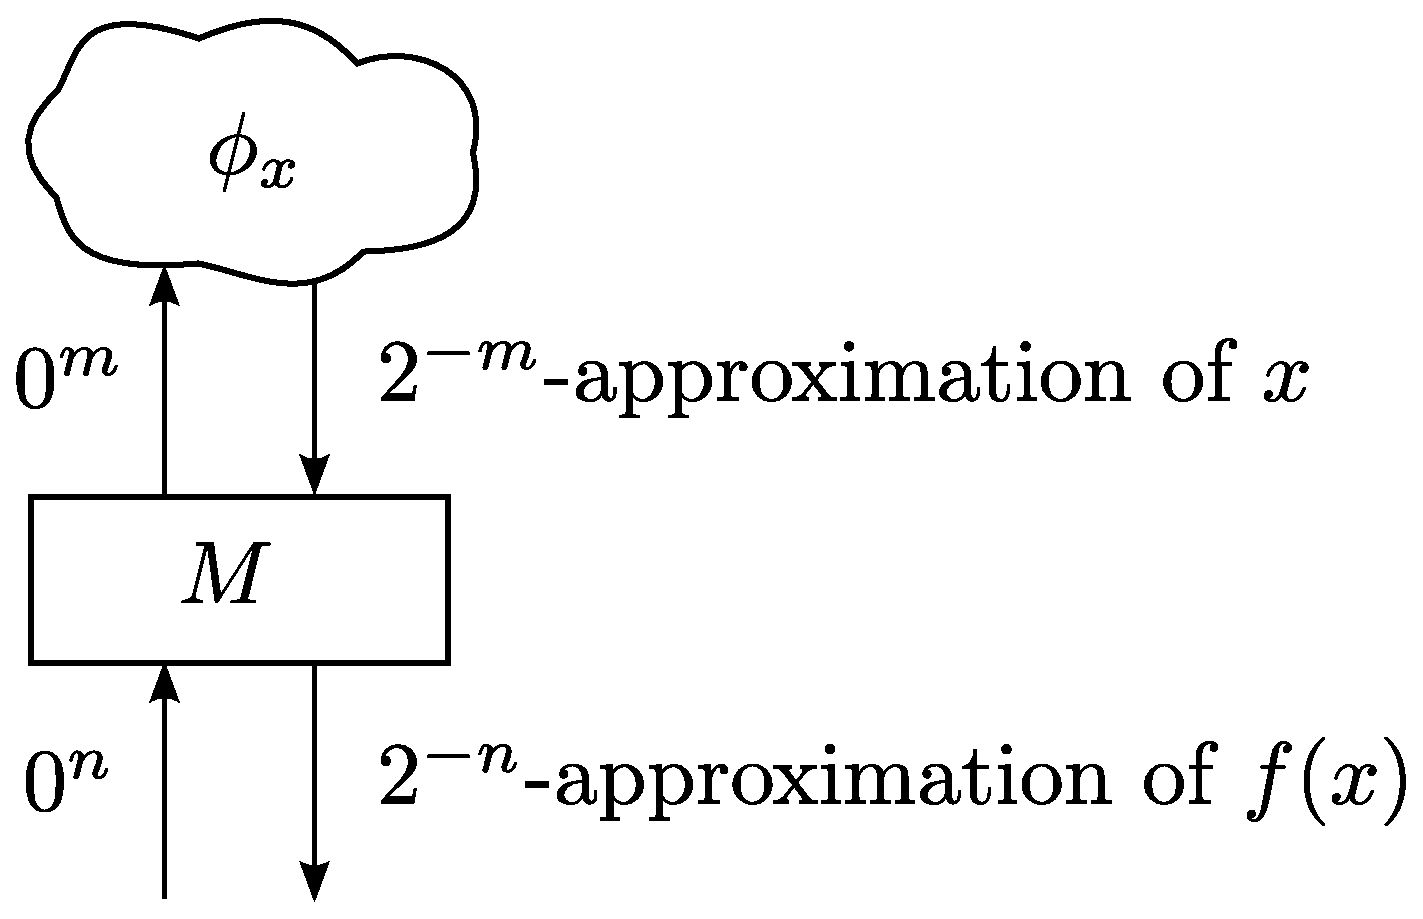
\includegraphics[height=0.15\textheight]{image/model-of-function.eps}
  \end{center}
  \caption{実関数を計算する機械}
  \label{fig:model-of-function}
 \end{figure}

機械$M$に, 
文字列から文字列への関数$\phi$を神託として与え, 
文字列$0 ^n$を入力として与えたとき, 
出力される文字列を$M ^\phi (0 ^n)$で表す. 
つまり$M ^\phi$をやはり文字列から文字列への関数とみる. 

\begin{definition}
$A$を$\R$の有界閉区間とする. 
機械 $M$ が実関数 $f \colon A \to \R$ を計算するとは,
任意の実数 $x \in A$, 任意の $x$ の名 $\phi_x$ に対して,
$M^{\phi_x}$ が $f(x)$ の名であること.
\end{definition}

$A$ が $\R ^2$ の有界閉領域であるときにも, 
神託を二つ取る機械を考えて同様に定義する. 


 ある実関数が\emph{計算可能}であるとは, その関数を計算する神託機械が存在することである.
 同様に, ある実関数が\emph{多項式時間計算可能}であるとは, その関数を計算する多項式時間神託機械が存在することである.

文字列$u$で添字づけられた実関数$f _u \colon A \to \R$の
族 $(f_u)_u$ を機械 $M$ が計算するとは,
任意の実数 $x \in A$, 任意の $x$ の名 $\phi_x$ に対して,
文字列 $v$ を $M ^{\phi _x} (u, v)$ へ移す関数が, 
$f _u (x)$ の名であることをいう.
 実関数族が多項式時間計算可能であるとは, その実関数族を計算する
 多項式時間神託機械が存在することである.

 神託機械 $M$ で $f$ を計算するとき, 求める精度 $n$ に対して,
 $x$ の近似値に必要な精度 $m$ が定まるため,
 計算可能な関数は連続である.
 また $n$ と $m$ の対応関係と有理数における近似値を与えることで,
 計算可能実関数や多項式時間計算可能実関数に対して,
 神託機械を用いない同値な特徴付けが可能である.

\begin{lemma}
  \label{lem:type1representation}
  実関数 $f\colon [0,1] \to \R$ に対して,
  $f$ が多項式時間計算可能であることは, 
  多項式時間計算可能な
  二つの関数 $\phi \colon (\Q \cap [0, 1]) \times \T \to \Q$ と
  $p \colon \N \to \N$ とが存在し, 
  任意の $d \in \Q \cap [0,1]$, $n \in \N$ について
  \begin{equation}
   |\phi(d, 0^n) - f(d)| \le 2^{-n} 
  \end{equation}
  任意の $x, y \in [0, 1]$, $m \in \N$ について
  \begin{equation}
   |x-y| \le 2^{-p(m)} \Rightarrow |f(x) - f(y)| \le 2^{-m} 
  \end{equation}
  が成立つことと同値である. 
\end{lemma}



\subsection{困難性}

 実関数の計算量の下界を述べるために, 困難性を定義する.

 まず実関数に言語が還元することを定義する.
 言語 $L \colon \{0, 1\} ^* \to \{0, 1\}$ が
 実関数 $f\colon [0,1] \to \R$ に多項式時間還元可能であるとは,
 $f$ を計算する機械を使って $L(u)$ を多項式時間で計算可能であることである.
 つまり $f$ を計算する機械があるとしたとき, 入力 $u$ に対して,
 精度 $n$ をこの機械に与え, ある実数 $x_u$ の神託を模倣し, $f(x_u)$ の $n$ 桁近似値から,
 $u$ が $L$ に属するか否かを多項式時間で計算可能であることである
 [図 \ref{fig:reduction}].
 厳密には以下のように定義する.

 \begin{definition}[多項式時間還元可能]
  言語 $L$ が実関数 $f\colon [0,1] \to \R$ に\emph{多項式時間還元可能}であるとは, 
  多項式時間計算可能な関数 $R,S,T$ が存在し, 
  任意の文字列 $u$ に対して以下を満たすことをいう. 
  \begin{itemize}
   \item $S(u, \cdot)$ はある実数 $x_u$ の名
   \item $f(x_u)$ の任意の名 $\phi$ に対して
	 \[
	  L(u) = R(u, \phi(T(u))).
	 \]
  \end{itemize}
 \end{definition}
 以下単に言語が実関数に還元可能といった場合, 多項式時間還元可能を指す.
 計算量 $C$ に対して, 関数 $f$ が \emph{$C$ 困難}であるとは,
 $C$ に属する任意の言語が $f$ に還元可能であることと定義する.

 \begin{figure}
  \begin{center}
  \label{fig:reduction}
  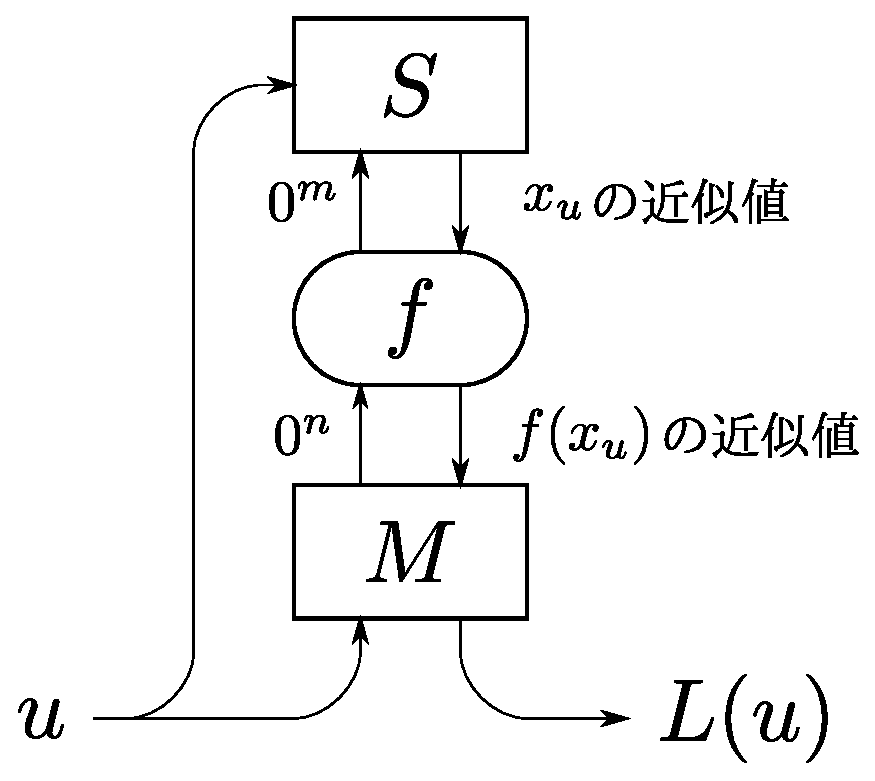
\includegraphics[scale=0.25]{image/reduction.eps}
  \caption{言語 $L$ から関数 $f$ への還元}
  \end{center}
 \end{figure}



